% This LaTeX template is intended for the students of CSI Master from
% University of Bordeaux to make their reports.
%
% This template can be used and modified with no restriction.
%
% %%% History %%%
%
% * April 22, 2014: First version (Emmanuel Fleury <fleury@labri.fr>)
%
% %%% Tips and Tricks %%%
%
% --- The memoir LaTeX class ---
% This template use the 'memoir' class, for more information about
% customization of this class see: http://www.ctan.org/pkg/memoir
%
% --- Rubber ---
% The Makefile are using the Rubber tool, install the 'rubber' package 
% to use it properly.
%

\documentclass[oneside]{memoir}
%\documentclass[a4paper]{memoir}

%%%%% Packages %%%%%
\usepackage{lmodern}
\usepackage{palatino}
\usepackage[T1]{fontenc}
\usepackage[utf8]{inputenc}

% To be removed if you want it in english
\usepackage[french]{babel}

\usepackage{amstext,amsmath,amssymb,amsfonts}
\usepackage{multirow,colortbl}
\usepackage{xspace,varioref}
\usepackage{hyperref}

\usepackage[dvipsnames]{xcolor}
\usepackage{graphicx}

\usepackage{appendix}
\usepackage{makeidx}

%% custom style %%%%%%%%%%%%%%%%%%%%%%%%%%%%%%%%%%%%%%%%%%%%%%%%%%%%%%%%

% custom commands
\newcommand{\version}[1]{\def\theversion{#1}}
\newcommand{\subtitle}[1]{\def\thesubtitle{#1}}

\newcommand{\authors}[1]{\def\theauthors{#1}\author{#1}}
\newcommand{\supervisor}[1]{\def\thesupervisor{#1}}
\newcommand{\tutor}[1]{\def\thetutor{#1}}

% translation for custom words
\newcommand{\authorname}{Authors}
\newcommand{\authorsname}{Authors}
\newcommand{\supervisorname}{Supervisor}
\newcommand{\tutorname}{Tutor}

\newcommand{\thepartname}{Part}

\ifdefined\addto{%
\addto{\captionsfrench}{\renewcommand{\authorname}{Auteur}}%
\addto{\captionsfrench}{\renewcommand{\authorsname}{Auteurs}}%
\addto{\captionsfrench}{\renewcommand{\supervisorname}{Superviseur}}%
\addto{\captionsfrench}{\renewcommand{\tutorname}{Tuteur}}}
\addto{\captionsfrench}{\renewcommand{\thepartname}{Partie}}
\else{}
\fi


%%%%% Setting Titlepage %%%%%
%%%%%%%%%%%%%%%%%%%%%%%%%%%%%
\pretitle{\flushleft\Huge\textsf}
\posttitle{\\[-.65em]\rule{\linewidth}{1.5mm}\\[-.65em]
\ifx\thesubtitle\undefined%
\else%
  \hfill{\small\itshape \thesubtitle}%
\fi
\centering
\vfill

\includegraphics{Universite_de_Bordeaux.pdf}
\vfill
\iflanguage{french}{%
 % {\Huge\bfseries Mémoire de fin d'étude}
{\Huge Projet de deuxième année}
% {\Huge Projet de première année}
}{%
  {\Huge Master Thesis}
% {\Huge Master2 Project}
% {\Huge Master1 Project}
}\\
\vspace{1.25em}
\iflanguage{french}{%
  \LARGE
  Master \emph{Sciences et Technologies},\\
  Mention \emph{Informatique},\\
% Mention \emph{Mathématiques},\\
  Parcours \emph{Cryptologie et Sécurité Informatique}.\\
  \par\hfill%
}{%
  \LARGE
  Master in \emph{Sciences and Technologies},\\
  Specialty in \emph{Computer Science},\\
% Specialty in \emph{Mathematics},\\
  Track \emph{Cryptology and Computer Security}.\\
  \par\hfill
}}

%% author
\preauthor{\vspace{\fill}\\
\ifx\theauthors\undefined%
  \flushleft\textbf{\large\authorname}\\
\else%
  \flushleft\textbf{\large\authorsname}\\
\fi
\small}
\postauthor{\vspace{1em}
\ifx\thesupervisor\undefined%
\else%
  \newline\textbf{\large\supervisorname}\\\thesupervisor\\[1em]%
\fi
\ifx\thetutor\undefined%
\else%
  \textbf{\large\tutorname}\\\thetutor%
\fi
\\[-.25em]
\rule{\linewidth}{1mm}\\[-.25em]}

%% version and date
\predate{\hspace{\fill}
\ifx\theversion\undefined%
\else%
  version~\theversion~--~%
\fi}
\postdate{}

%% chapters style %%%%%%%%%%%%%%%%%%%%%%%%%%%%%%%%%%%%%%%%%%%%%%%%%%%%%%
%% You may try several styles (see more in the memoir manual).

%\chapterstyle{veelo}
%\chapterstyle{chappell}
%\chapterstyle{ell}
%\chapterstyle{ger}
%\chapterstyle{pedersen}
%\chapterstyle{verville}
%\chapterstyle{madsen}
\chapterstyle{thatcher}

%% parts style %%%%%%%%%%%%%%%%%%%%%%%%%%%%%%%%%%%%%%%%%%%%%%%%%%%%%%%%%

\renewcommand*{\thepart}{\arabic{part}}

\renewcommand*{\parttitlefont}{\chaptitlefont\Huge}
\renewcommand*{\partnamefont}{\chapnamefont\HUGE}
\renewcommand*{\partnumfont}{\chapnumfont\HUGE}

\renewcommand{\beforepartskip}{\vspace*{\fill}}
\renewcommand{\midpartskip}{\vspace{.5em}\hrule height 1.5mm \vspace{.5em}}
\renewcommand{\afterpartskip}{\vspace*{\fill}}

% table of contents
\renewcommand*{\cftpartname}{\thepartname}
\renewcommand*{\cftpartpresnum}{\space}
\renewcommand*{\cftpartaftersnum}{.}
\renewcommand*{\cftpartaftersnumb}{\space}

\cftpagenumbersoff{part}
\renewcommand{\cftpartafterpnum}{\protect\\[-.75em]%
  \protect\mbox{}\protect\hrule\par}

\renewcommand{\cftchapterdotsep}{4}


%% index generation %%%%%%%%%%%%%%%%%%%%%%%%%%%%%%%%%%%%%%%%%%%%%%%%%%%%
\makeindex

%%%%% Useful macros %%%%%
\newcommand{\latinloc}[1]{\ifx\undefined\lncs\relax\emph{#1}\else\textrm{#1}\fi\xspace}
\newcommand{\etc}{\latinloc{etc}}
\newcommand{\eg}{\latinloc{e.g.}}
\newcommand{\ie}{\latinloc{i.e.}}
\newcommand{\st}{\ensuremath{\text{\xspace s.t.\xspace}}}


%%%%% Report Title %%%%%
\title{Single Packet Authorization}
%\subtitle{Le sous-titre du rapport (optionnel)}

% If only one author use \author
\author{Jean Dupont \texttt{<jean.dupont@etu.u-bordeaux.fr>}}

% If several authors use \authors{}
\authors{Cédric Ceola \texttt{<cedric.ceola@etu.u-bordeaux.fr>}\\
Jacques Monin \texttt{<jacques.monin@etu.u-bordeaux.fr>}\\}

%\supervisor{Jane Doe \texttt{<jane.doe@mycompany.com>}}

\tutor{Abdou Guermouche \texttt{<abdou.guermouche@u-bordeaux.fr>}}

%\version{0.1}

%%%%% Document %%%%%
%%%%%%%%%%%%%%%%%%%%
\begin{document}

\frontmatter%%%%%%%%%%%%%%%%%%%%%%%%%%%%%%%%%%%%%%%%%%%%%%%%%%%%%%%%%%%%
\maketitle
\clearpage

\tableofcontents*

\chapter*{Introduction}

Afin d'empêcher le scan de port d'un pare-feu protégeant un serveur applicatif, de nombreuses techniques ont vu le jour. En effet, posséder un pare-feu dont tous les ports sont fermés et ne s'ouvrent que lors d'échanges avec des clients approuvés permettrait d'amoindrir les attaques sur ce serveur.

Le but est donc de fermer par défaut les ports logiciels du pare-feu et mettre en place un mécanisme de reconnaissance des clients autorisés à interagir avec le serveur.

De plus, il existe une restriction supplémentaire qui est que le client doit pouvoir faire ouvrir un port au serveur via un unique paquet envoyé.

Plusieurs modèles ont tentés de répondre à cette question, nous allons étudier les plus connus.


\mainmatter%%%%%%%%%%%%%%%%%%%%%%%%%%%%%%%%%%%%%%%%%%%%%%%%%%%%%%%%%%%%%
\part{Deux modèles d'ouverture de port dynamique}

\chapter{Port Knocking}

Le Port Knocking est un des modèles qui a été inventé pour répondre au besoin d'ouverture et de fermeture automatique de ports.

Dans ce modèle, la client s'authentifie auprès du serveur en lançant des tentatives de connexions sur certains ports spécifiques constituant un code. Le serveur ouvre un port seulement si le même émetteur réalise la bonne séquence de tentative de connexion.

Cette solution nécessite peu de ressource et est aisée à mettre en place, cependant une simple écoute du réseau permet de repérer le code permettant l'ouverture d'un port ce qui rend cette solution facilement attaquable.

\chapter{Single Packet Authorization}

Le Single Packet Authorization est le second modèle qui répond à cette problématique. Ce mécanisme repose sur l'envoi, par le client, d'une unique requête au pare-feu.

En suivant ce système, le client va envoyé cette requête contenant un numéro de port. Le pare-feu laissera ensuite passé les paquets émis par le client, à destination du serveur applicatif en utilisant ce port et ce pour une période limitée.

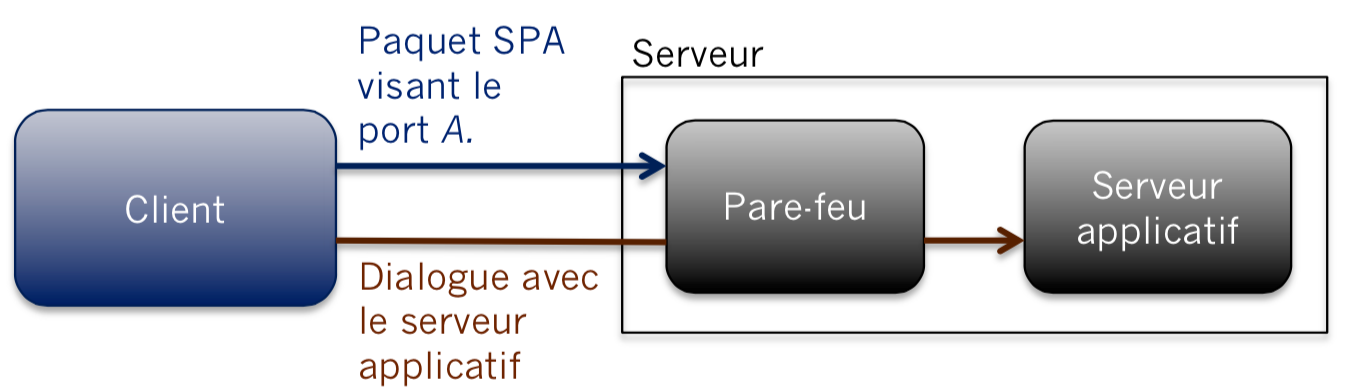
\includegraphics[scale=0.5]{spa_general_1}

Afin que ce mécanisme soit sécurisé, le pare-feu possèdera une clé spécifique à chaque client garantissant ainsi qu'aucune identité ne pourra être usurpée.

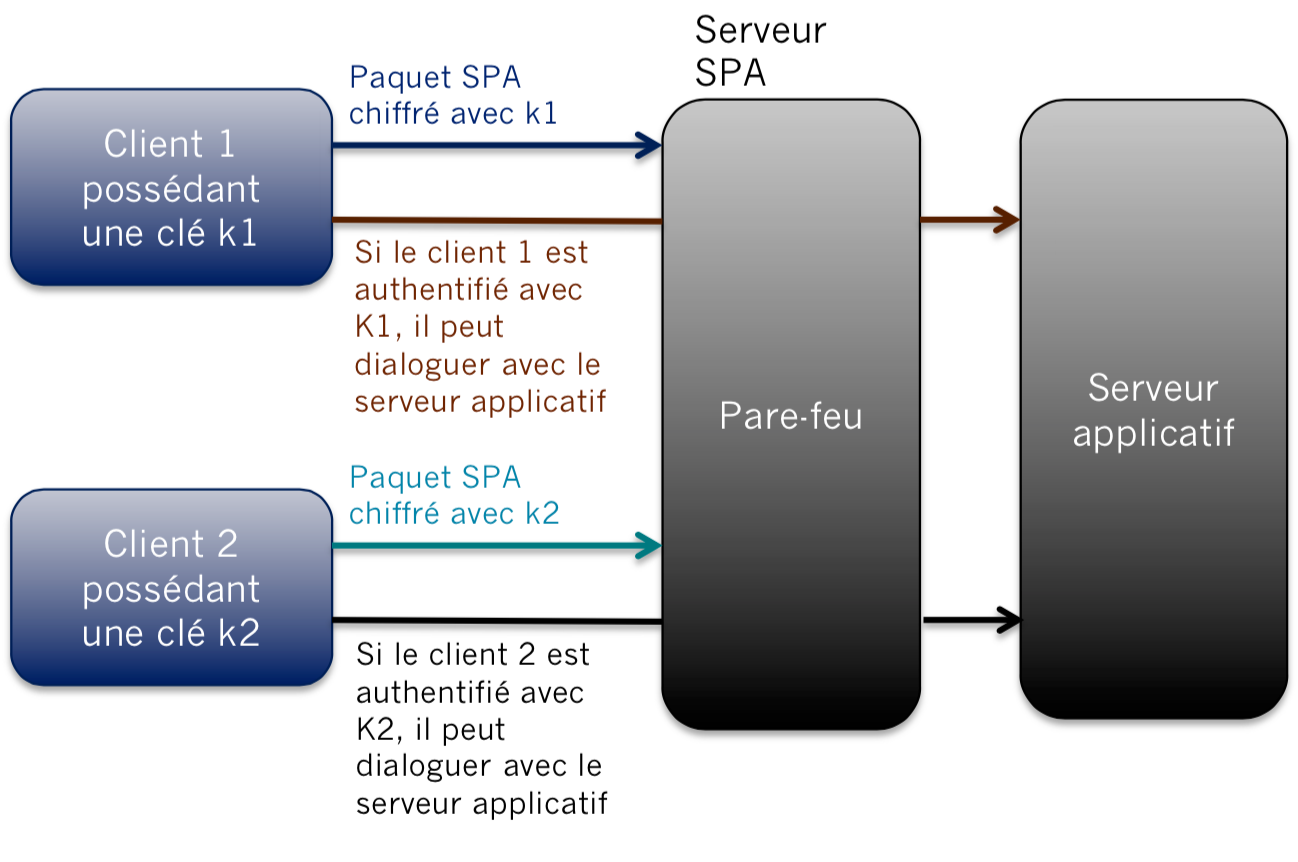
\includegraphics[scale=0.5]{spa_general_2}

Grâce à des principes supplémentaires expliqués ultérieurement, il sera possible d'empêcher des attaques de type rejeu.

Nous nous proposons d'étudier plus en profondeur cette méthode.


%%%%%%%%%%%%%%%%%%%%%%%%%%%%%%%%%%%%%%%%%%%%%%%%%%%%%%%%%%%%%%%%%%%%%%%%
\part{Réalisation de SPA}
\clearpage
Dans le cadre de notre étude du SPA, nous avons programmé un couple client serveur pour répondre aux exigences demandées par l'ouverture de ports dynamique.

Nous allons vous présenter les différentes étapes que nous avons traversées pour rendre le programme robuste, c'est à dire afin que seul un client puisse ouvrir un port du firewall pour un court laps de temps.

Ci-dessous un schéma de la topologie réseau mise en place.

/!\\ Insérer schéma

4 machines sont présentes, le client SPA, le serveur SPA, un attaquant en man-in-the-middle et le serveur applicatif avec lequel le client veut discuter.

Le but est donc l'ouverture d'un port du firewall situé sur la machine qui possède le serveur SPA via l'envoie d'un unique paquet SPA venant du client. L'attaquant qui voit l'intégralité de la communication entre le client et le serveur (qui est unilatérale) doit être incapable d'utiliser ces informations à son avantage.

Pour cela, il est nécessaire de préserver l'intégrité et l'authenticité des données transmises au serveur SPA. En effet, l'attaquant ne doit pas pouvoir se faire passer pour le client sinon il aura la capacité de faire ouvrir au serveur des ports du pare-feu.
De plus, l'intégrité des données doit aussi être préservée puisqu'il ne faut pas qu'un attaquant change les spécifications du client, il pourait sinon changer le numéro de port ouvert par exemple par un qui l'interesserait plus.
 

\chapter{Authenticité et Intégrité}
Après avoir présenté le procédé, nous allons détailler davantage les outils utilisés pour le satisfaire.

Pour palier à la faiblesse du \emph{Port Knocking}, et afin qu'une simple écoute du réseau ne suffise pas à mettre en péril ce schéma, la pérénnité de cette méthode va reposer sur l'authentification des clients. En effet il est nécessaire de vérifier que l'acceptation d'un paquet par le pare-feu est bien effectuée par un client légitime.

A contrario du \emph{Port Knocking} qui supposait que seul un client autorisé pouvait connaître la séquence de coups, ici l'authenticité va se faire grâce à des clés prépartagées. En effet, le serveur va partager une clé avec chacun des ses clients, chaque clé étant différente des autres. 
Le client génère alors un paquet SPA chiffré avec cette clé, le serveur SPA le déchiffre avec la même clé. Il détermine la légitimité de la requête et si les champs sont valides, l'intégrité grâce au système de hachage

Si la demande est valide, le client sera considéré comme authentifié auprès du serveur et il pourra communiquer avec lui sur le port fourni.

\section{Chiffrement}

Pour le chiffrement, nous utiliserons le standard du chiffrement symétrique, AES. 
Pour choisir le mode d'opération cryptographique, nous avons du choisir entre plusieurs modes. 
Sachant que nos données à chiffrer sont de taille limitée, nous n'utiliserons pas un mode de chiffrement qui se comporte comme un chiffrement par flux.
De plus, nous savons que ECB connait des vulnérabilités quant à l'intégrité et la protection des données puisqu'il est sensible aux attaques par répétition (deux blocs avec le même contenu seront chiffrés de la même manière).
%Par ailleurs, OFB est fragile vis-à-vis des attaques à clair connu et CTR est fragile si l'attaquant connait l'IV (ce qui sera le cas ici étant donné que celui-ci sera envoyé en clair).
Nous choisirons donc CBC.


Nous désirons que le client puisse choisir le port serveur avec lequel il veut communiquer, le protocole de transport utilisé (tcp ou udp) ainsi que le temps d'accès au port (en maintenant un temps maximal d'ouverture de port).

\section{Champ \textbf{\emph{IP}} du paylaod}

De plus, afin de s'assurer de l'authenticité de l'émetteur du paquet, celui-ci doit introduire son adresse IP dans le champ de données chiffré. Ainsi, en comparant cette donnée et le header du paquet ip, il sera possible de voir si les informations sont cohérentes et donc authentiques (un attaquant n'étant pas en mesure de fournir un chiffré valide sans la clé adéquate). 
un Utilisateur légitime construit naturellement un paquet avec ces deux champs IP identiques. Un usurpateur pourra alors être démasqué si sa requête ne respecte pas cela.

\section{Hachage}
\begin{quotation}
\emph{"Une fonction de hachage [...] doit être rapide à calculer, transforme un message de longueur arbitraire en une empreinte numérique de taille fixe. Cette dernière est ensuite signée ..."}
\end{quotation}
\underline{\emph{Codage, cryptologie et applications}}, \textbf{Bruno Martin}\\

l'intérêt des fonctions de hachage est de vérifier l'intégrité du champ de donnée et nous rendons le haché authentique grâce au chiffrement par AES.
Il nous faut maintenant déterminer quel algorithme est le plus adapté sachant que les plus courant sont MD5, SHA1, SHA-256 ou SHA-512.\newline

Le système MD5, était considéré comme sûr avant que les chercheurs chinois, \emph{Xiaoyun Wang, Dengguo Feng, Xuejia Lai (co-inventeur de IDEA) et Hongbo Yu "} ne soient capables de trouver des collisions en quelques heures et le brisent.
le système SHA-1 est, lui aussi, sensible aux collisions notamment à celles basées sur le paradoxe des anniversaires.
Nous avons donc choisi SHA-256 plutôt que SHA-512 pour la taille restreinte du haché produit tout en sachant que le réel intérêt de ce haché est d'établir une simple somme de contrôle.\newline

Nous hachons tous les champs de données de la requête et la concaténons à ceux-ci puis le tout sera chiffré afin de préserver l'intégrité des informations. Si le chiffré est changé, le haché ne correspondra plus aux champs de donnée.

Nous avons mis en place un système permettant d'authentifier les requêtes arrivant au serveur SPA ainsi que vérifier l'intégrité de celles-ci, nous allons maintenant nous intéresser à contrer certains attaques supplémentaires.
 %http://fr.wikipedia.org/wiki/MD5
 
 

\chapter{Protection contre Rejeu et DDoS}

\section{Rejeu}

Dans un contexte de Single Packet Autorization, il est indispensable de vérifier qu'un paquet n'est pas issu du rejeu.

En effet, à ce stade, il est possible pour un attaquant qui écoute le réseau d'enregistrer un paquet envoyé par un client légitime et le renvoyer dès qu'il souhaite une ouverture de port. Nous allons proposer deux solutions pour résoudre ce problème.

\subsection{Détection par Horodatage}

Dans le but de résoudre ce problème, il est possible d'utiliser un horodatage. Le client envoie les informations précédemment présentées auxquelles sont ajoutées l'année, le mois, le jour et l'heure de création du paquet. Le serveur a une structure gérant le rejeu où il enregistrera, entre autres, l'heure de fermeture du port et le hachage du chiffré reçu. Lorsque l'heure de fermeture du port est arrivée, le paquet sort de la structure.

Deux possibilités d'attaques s'offrent à nous :

\begin{itemize}

\item L'attaquant rejoue un paquet alors que la règle du pare-feu est toujours active. Le serveur remarque que ce paquet a déjà été reçu puisque son haché est dans la structure.

\item L'attaquant rejoue un paquet alors que la règle du pare-feu n'est plus active. Le serveur remarque que l'heure de la création du paquet ajouté au temps d'ouverture du port (donnant l'heure de fermeture du port) est déjà passée, ce paquet est donc ignoré.

\end{itemize}

\vspace{0.5cm}

\subsection{Détection par les \textbf{O}ne-\textbf{T}ime-\textbf{P}assword}

Une autre manière de faire est l'utilisation des One-Time-Password. Ces outils cryptographiques permettent de faire évoluer un mot de passe statique afin que pour chaque chiffrage/déchiffrage, une clé différente soit utilisée. Ainsi, renvoyer un paquet qui a été chiffré avec une certaine clé et qui a déjà été reçu par le serveur sera déchiffré avec une autre clé et ne sera donc pas traité.

C'est une mécanisme d'authentification forte puisqu'en plus de la graine que le serveur et le client partagent, ils devront avoir en commun un secret supplémentaire.\\

Pour cela, plusieurs types d'OTP existent basés sur:

\begin{itemize}

\item \textbf{l'utilisation d'un compteur} : le client et le serveur partagent un compteur en commun. Ce compteur évolue à chaque authentification.

\item \textbf{l'utilisation du temps} : le mot de passe créé à partir de la graine et de l'heure courante n'est valable que pendant une certaine durée.

\item \textbf{l'utilisation de challenge} : le serveur communique des données aléatoire au client qui va créer l'OTP à partir de celui-ci. Une challenge sera envoyé pour chaque nouvel OTP.

\end{itemize}

\vspace{0.5cm}

Dans le cadre du SPA, il faut qu'il n'y ait pas d'autre dialogue entre le client et le serveur SPA que celui déjà connu. Nous n'utiliserons pas l'OTP basé sur les challenges.

Nous avons choisi d'utiliser des compteurs (H-MAC Based OTP). Le client et le serveur partagent une graine et un compteur, le mot de passe courant sera le résultat du hmac entre ces deux valeurs. A chaque nouveau paquet, le compteur évoluera.

Ainsi, si un attaquant rejoue un paquet, celui-ci sera déchiffré avec la clé courante du serveur qui n'est pas celle qui a servi à déchiffrer le paquet rejoué. Celui-ci ne sera donc pas traité et le compteur du serveur n'évoluera pas pour rester synchronisé avec le client.

\clearpage

\section{DoS et DDoS}

Les attaques de type déni de service ont pour but de rendre un service inaccessible voire entraîner son arrêt.

Ces attaques peuvent être distribuées, c'est à dire que les origines de cette attaque sont multiples.

Pour contrer une attaque de déni de service, le serveur n'accepte pas plus d'un certain nombre de requêtes de la part d'un même client. Un unique client ne pourra donc pas saturer le serveur, toute requête supplémentaire de sa part ne sera pas traitée.

Il n'est pas possible d'empêcher de rendre un service inaccessible lors d'une attaque de déni de service distribué, cependant, dans le but d'empêcher le plantage du serveur, un nombre total de requêtes traitées a été mis en place.


%%%%%%%%%%%%%%%%%%%%%%%%%%%%%%%%%%%%%%%%%%%%%%%%%%%%%%%%%%%%%%%%%%%%%%%%
\part{Implémentation et évolution}
\clearpage

\chapter{Implémentation}

Pour mettre en place cette méthode, nous avons développé une paire client-serveur SPA en langage C.

La topologie utilisée lors du développement et des tests est un réseau de 4 machines virtuelles : 

\begin{figure}[h]

\centerline{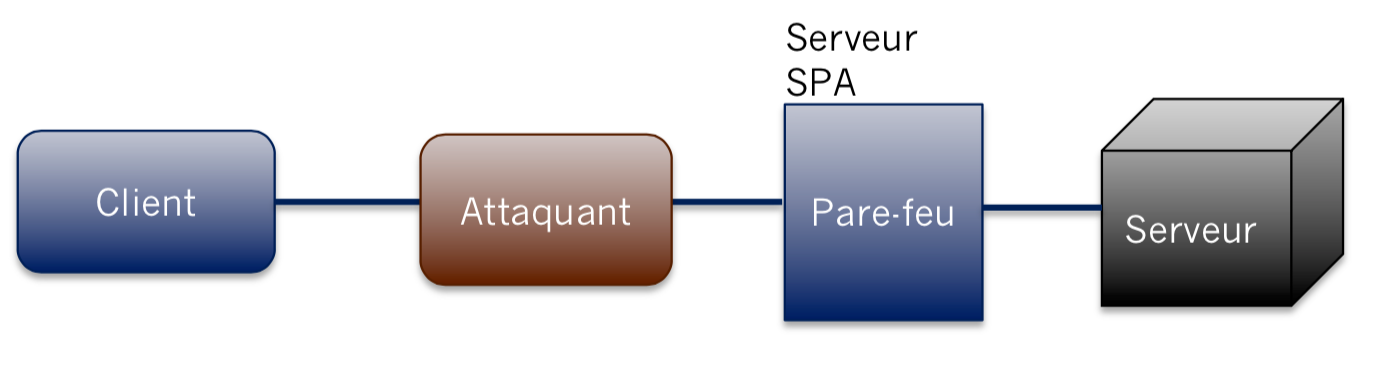
\includegraphics[scale=0.5]{topo_imple}}
\caption{Topologie du réseau de machines virtuelles}

\end{figure}
Nous avons ainsi fait appel à diverses librairies dont nous allons détailler l'intérêt.

\subsection{Libnet}
Dans un premier temps, nous avons eu besoin d'envoyer un paquet depuis le client vers le serveur, pour cela nous avons utilisé la librairie \emph{Libnet} qui nous a permis de mettre en place une socket RAW, de créer l'encapsulation IP, UDP et de placer les données à envoyer.

\subsection{Open SSL}
Afin d'authentifier cette demande, nous avons utilisé la librairie \emph{OpenSSL} possédant une documentation complète (voir bibliographie).
Les HMAC Based OTP, eux aussi, sont gérés grâce à la librairie \emph{OpenSSL}. Plus précisément, nous avons utilisé la fonction de calcul \emph{HMAC} qu'elle contient.

\subsection{Libpcap}
Pour récupérer ce paquet depuis le serveur, nous avons utilisé la librairie \emph{libpcap} qui nous a permis de filtrer les paquets afin de récupérer les \emph{SPA}. Nous avons pu différencier ces paquets grâce au fait qu'ils ont pour destination un port unique du pare-feu. Nous traitons ensuite ces requêtes une par une.

\subsection{Time.h}
Pour assurer une bonne gestion de l'horodatage aux client et au serveur SPA, nous avons utilisé la bibliothèque time.h
 afin de s'assurer que le temps utilisés ne pâtissent pas de problème de fuseaux horaires.

\subsection{LibXML2}

Enfin, nous avons, à l'aide de la librairie \emph{LibXML2}, enregistré les informations nécessaires à l'utilisation de HOTP dans un fichier \emph{XML} (au niveau client et serveur).
Ce fichier contient :
\begin{itemize}
\item \textbf{Au niveau du serveur SPA} ,une entrée par client authentifié. Dans cette entrée sont stockés la graine (secret partagé), le compteur et un identifiant (ici une adresse IP) permettant au serveur de différencier ses clients.
\item \textbf{Au niveau du client}, une seule entrée contenant le secret partagé et un compteur ayant, au temps \emph{t}, la même valeur pour le client et le serveur.
\end{itemize}

\subsection{Structure de connections actives}

Contrairement au fichier XML, nous souhaitons que le serveur garde en mémoire les connections actives. Nous utilisons donc une structure qui contient la liste des clients authentifié possédant en même temps une autorisation de communication particulière avec le serveur applicatif. Nous avons ainsi implémenter une liste chaînée contenant, dans chaque cellule, des informations sur la connexion et sur le client qui en est à l'origine tout en permettant d'ajouter, de modifier ou de supprimer une entrée.

\chapter{Tests}

\section{Utilisation du client-serveur}

Nous nous proposons de tester notre implémentation. Nous allons essayer de nous connecter en ssh depuis le client sur le serveur applicatif ceci en utilisant la méthode SPA.

Nous allons depuis la machine client tenter une connexion ssh vers le serveur applicatif en 10.0.0.2

\begin{figure}[h]

\centerline{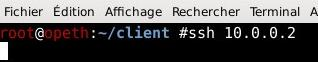
\includegraphics[scale=0.75]{test_ssh.jpeg}}

\end{figure}

Celle-ci ne fonctionne pas car les règles du pare-feu ne laissent pas passer la connexion.

\begin{figure}[h]

\centerline{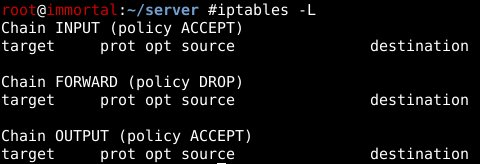
\includegraphics[scale=0.6]{regles_ip_avant}}

\end{figure}

Pour parrer à ces restrictions, nous allons envoyer un paquet SPA demandant de laisser passer les communications en tcp vers le port 22.

\begin{figure}[h]

\centerline{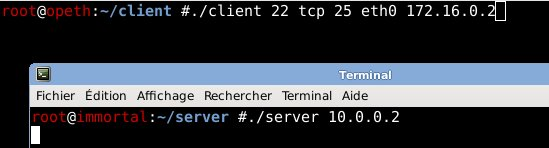
\includegraphics[scale=0.6]{execution_client.jpeg}}

\end{figure}

Voici ce que nous pouvons voir sur le serveur après réception du paquet.
\clearpage

\begin{figure}[h]

\centerline{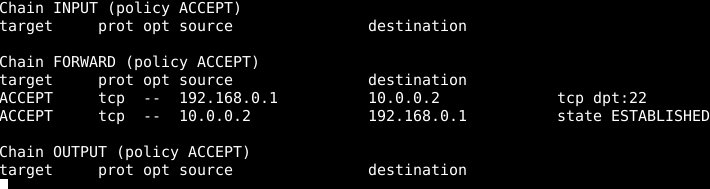
\includegraphics[scale=0.7]{regles_apres.jpeg}}

\end{figure}

La connexion ssh fonctionne maintenant (mais seulement pour le temps spécifié).

\begin{figure}[h]

\centerline{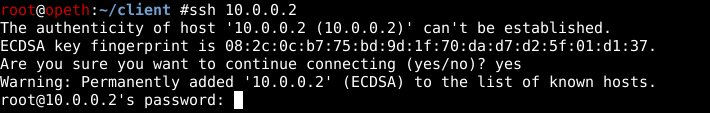
\includegraphics[scale=0.6]{test_ssh2.jpeg}}

\end{figure}

25 secondes plus tard, les règles iptables sont supprimées et la connexion n'est plus possible.

\clearpage
\section{Attaques}

Mettons-nous à la place de l'attaquant. En écoutant sur le réseau, nous retrouvons le paquet SPA formé de cette manière. On se rend compte que toutes les données sont chiffrées et qu'il n'y a que l'IV à la fin du message en clair.

\begin{figure}[h]

\centerline{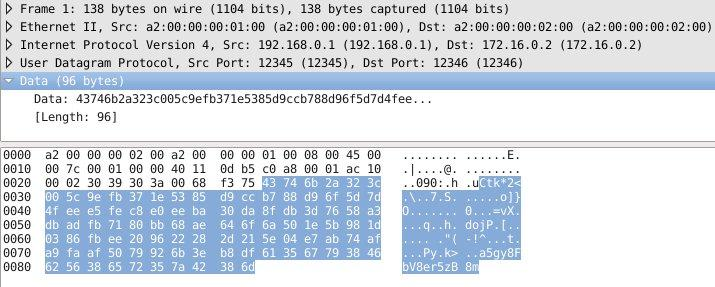
\includegraphics[scale=0.6]{wireshark.jpeg}}

\end{figure}

En essayant de rejouer un paquet sur le réseau, le serveur le détecte en n'en tient pas compte.

\begin{figure}[h]

\centerline{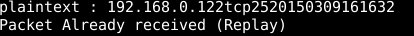
\includegraphics[scale=0.8]{rejeu.jpeg}}

\end{figure}

\chapter{Perspectives d'évolution}

Nous avons vu que notre implémentation satisfaisait un fonctionnement de base du principe de SPA.
Cependant, nous avons noté quelques perspectives d'amélioration qui rendraient le tout plus robuste et complet.

\section{Mise à jour des OTP}
Dans une précédente partie, nous avons détaillé le choix de notre système de gestion des clefs a usages unique. 
Celles-ci sont générées par une \emph{seed} et un compteur qui évolue à chaque envoie d'un paquet SPA.
Nous faisons actuellement évoluer ce compteur de façon analogue pour chaque client.
Ainsi, la connaissance à un moment donné de la \emph{seed} et du compteur pourrait permettre à n'importe quel autre partie ayant conscience du mécanisme d'évolution du compteur de déterminer la clef suivante.

\section{Appel a la librairie Libnetfilter}
En ce qui concerne l'intéraction concrète avec les règles iptables du pare-feu, nous utilisons des appels systèmes simples. Cependant, l'utilisation de librairies plus spécifiques telles que \emph{libnetfilter} pourrait sembler plus adapté.
\chapter*{Conclusion}

Faire conclusion


%%%%%%%%%%%%%%%%%%%%%%%%%%%%%%%%%%%%%%%%%%%%%%%%%%%%%%%%%%%%%%%%%%%%%%%%

%\part*{Annexes}
%\addcontentsline{toc}{part}{Annexes}
%\appendix

%\chapter{Dolor}

Lorem ipsum dolor sit amet, consectetur adipiscing elit. Fusce luctus
euismod nunc, quis tincidunt lorem egestas in. Nulla hendrerit vel
ante eu gravida. Vivamus eu dapibus libero. Vestibulum dolor tortor,
malesuada et leo et, luctus faucibus augue. Nullam dapibus, tortor non
vulputate rutrum, dolor risus posuere ligula, a tincidunt sapien velit
non odio. Pellentesque sit amet aliquet augue. Nam interdum nunc non
ornare dapibus. Aliquam congue vitae sapien non rutrum. Vestibulum
varius iaculis luctus. Donec vitae congue est. Nunc mattis libero sed
nisl vestibulum, ut vestibulum leo aliquet. Donec volutpat arcu
cursus, varius nunc sit amet, elementum mauris. Aenean auctor
facilisis ultrices. Nulla et magna mi. Ut pretium lacus et risus
tempor cursus.

 Cras sed magna ut nunc varius ornare. Sed sollicitudin porttitor
 metus, nec dignissim neque egestas non. Vestibulum suscipit
 sollicitudin pellentesque. Vivamus vehicula mauris faucibus fermentum
 viverra. Donec ac risus nec magna molestie ornare eu quis metus.
 Nulla eu erat quis mi eleifend volutpat et eu justo. Proin id ipsum
 in purus pellentesque tempor. Maecenas tristique tincidunt elit, quis
 rhoncus velit lobortis eu. Nunc sit amet nisi vehicula, varius massa
 nec, pellentesque nulla. Fusce porta mi ut vulputate vulputate. Fusce
 sed ornare tortor, gravida fermentum nibh.

Nullam imperdiet purus at arcu pretium faucibus. Quisque bibendum
velit enim, eu volutpat mauris lacinia sit amet. Nulla dictum posuere
urna sed tincidunt. Mauris eget lobortis turpis, vitae consequat
turpis. Pellentesque habitant morbi tristique senectus et netus et
malesuada fames ac turpis egestas. Etiam at dui ut neque accumsan
tempus. Suspendisse vitae dolor placerat, adipiscing nunc sit amet,
consectetur elit. Nam euismod augue eu consequat faucibus. Vivamus
rhoncus lorem fringilla quam sagittis, in facilisis ante ultrices.
Praesent elementum augue non odio pellentesque, eget euismod justo
volutpat. Integer convallis dignissim orci ac varius. Aenean cursus
metus vel risus fringilla cursus. Fusce vitae gravida nibh, semper
fringilla leo. Pellentesque lorem nunc, vehicula ut sapien et,
hendrerit luctus sem.

Nam nulla sapien, fermentum in lectus eu, rhoncus feugiat tortor. Sed
et arcu quis nibh egestas ultrices. Sed eu blandit libero. Suspendisse
et ultricies purus. Interdum et malesuada fames ac ante ipsum primis
in faucibus. Sed viverra, urna a adipiscing tristique, augue orci
ornare tellus, sed cursus mauris lacus sit amet magna. Integer
hendrerit laoreet tincidunt. Pellentesque varius condimentum purus ac
interdum. Nullam quam tortor, suscipit at porta in, laoreet nec nulla.
Ut varius ligula enim, in feugiat erat malesuada vitae. Nunc ligula
elit, iaculis nec lobortis eu, accumsan a justo. Maecenas volutpat
laoreet lorem. Phasellus fringilla lacus et dui fermentum sagittis.
Morbi vitae leo eget neque gravida egestas. Mauris dolor metus,
consectetur nec ultricies at, egestas quis ligula. Proin mollis nec
purus eget sollicitudin.

Sed quis ante ac quam semper pretium vitae at urna. Ut id mollis dui.
Duis venenatis ante vel justo lobortis laoreet. Nulla facilisi. Cras
massa massa, tristique cursus mattis non, luctus sed tellus. Morbi in
dui bibendum orci consequat gravida. Vestibulum sed augue et odio
posuere vehicula a ac odio. Ut eleifend, purus eget volutpat
tincidunt, orci ante malesuada dui, quis scelerisque metus dolor et
metus. Phasellus volutpat hendrerit egestas.

%\chapter{Sit}

Lorem ipsum dolor sit amet, consectetur adipiscing elit. Fusce luctus
euismod nunc, quis tincidunt lorem egestas in. Nulla hendrerit vel
ante eu gravida. Vivamus eu dapibus libero. Vestibulum dolor tortor,
malesuada et leo et, luctus faucibus augue. Nullam dapibus, tortor non
vulputate rutrum, dolor risus posuere ligula, a tincidunt sapien velit
non odio. Pellentesque sit amet aliquet augue. Nam interdum nunc non
ornare dapibus. Aliquam congue vitae sapien non rutrum. Vestibulum
varius iaculis luctus. Donec vitae congue est. Nunc mattis libero sed
nisl vestibulum, ut vestibulum leo aliquet. Donec volutpat arcu
cursus, varius nunc sit amet, elementum mauris. Aenean auctor
facilisis ultrices. Nulla et magna mi. Ut pretium lacus et risus
tempor cursus.

 Cras sed magna ut nunc varius ornare. Sed sollicitudin porttitor
 metus, nec dignissim neque egestas non. Vestibulum suscipit
 sollicitudin pellentesque. Vivamus vehicula mauris faucibus fermentum
 viverra. Donec ac risus nec magna molestie ornare eu quis metus.
 Nulla eu erat quis mi eleifend volutpat et eu justo. Proin id ipsum
 in purus pellentesque tempor. Maecenas tristique tincidunt elit, quis
 rhoncus velit lobortis eu. Nunc sit amet nisi vehicula, varius massa
 nec, pellentesque nulla. Fusce porta mi ut vulputate vulputate. Fusce
 sed ornare tortor, gravida fermentum nibh.

Nullam imperdiet purus at arcu pretium faucibus. Quisque bibendum
velit enim, eu volutpat mauris lacinia sit amet. Nulla dictum posuere
urna sed tincidunt. Mauris eget lobortis turpis, vitae consequat
turpis. Pellentesque habitant morbi tristique senectus et netus et
malesuada fames ac turpis egestas. Etiam at dui ut neque accumsan
tempus. Suspendisse vitae dolor placerat, adipiscing nunc sit amet,
consectetur elit. Nam euismod augue eu consequat faucibus. Vivamus
rhoncus lorem fringilla quam sagittis, in facilisis ante ultrices.
Praesent elementum augue non odio pellentesque, eget euismod justo
volutpat. Integer convallis dignissim orci ac varius. Aenean cursus
metus vel risus fringilla cursus. Fusce vitae gravida nibh, semper
fringilla leo. Pellentesque lorem nunc, vehicula ut sapien et,
hendrerit luctus sem.

Nam nulla sapien, fermentum in lectus eu, rhoncus feugiat tortor. Sed
et arcu quis nibh egestas ultrices. Sed eu blandit libero. Suspendisse
et ultricies purus. Interdum et malesuada fames ac ante ipsum primis
in faucibus. Sed viverra, urna a adipiscing tristique, augue orci
ornare tellus, sed cursus mauris lacus sit amet magna. Integer
hendrerit laoreet tincidunt. Pellentesque varius condimentum purus ac
interdum. Nullam quam tortor, suscipit at porta in, laoreet nec nulla.
Ut varius ligula enim, in feugiat erat malesuada vitae. Nunc ligula
elit, iaculis nec lobortis eu, accumsan a justo. Maecenas volutpat
laoreet lorem. Phasellus fringilla lacus et dui fermentum sagittis.
Morbi vitae leo eget neque gravida egestas. Mauris dolor metus,
consectetur nec ultricies at, egestas quis ligula. Proin mollis nec
purus eget sollicitudin.

Sed quis ante ac quam semper pretium vitae at urna. Ut id mollis dui.
Duis venenatis ante vel justo lobortis laoreet. Nulla facilisi. Cras
massa massa, tristique cursus mattis non, luctus sed tellus. Morbi in
dui bibendum orci consequat gravida. Vestibulum sed augue et odio
posuere vehicula a ac odio. Ut eleifend, purus eget volutpat
tincidunt, orci ante malesuada dui, quis scelerisque metus dolor et
metus. Phasellus volutpat hendrerit egestas.



\backmatter%%%%%%%%%%%%%%%%%%%%%%%%%%%%%%%%%%%%%%%%%%%%%%%%%%%%%%%%%%%%%

\nocite{*}
\bibliographystyle{plain}
\bibliography{bibliography}

\printindex

\end{document}
